\documentclass[11pt,a4paper]{article}
\usepackage[T1]{fontenc}
\usepackage[utf8]{inputenc}
\usepackage{amsmath,amsthm}
\usepackage{newtxtext,newtxmath}
\usepackage[a4paper,margin=19mm,top=22mm,bottom=22mm,headheight=14pt]{geometry}
\usepackage{amsmath,amsthm,booktabs,longtable,tabularx,array,microtype}
\usepackage{xcolor,graphicx,tikz,tcolorbox,fancyhdr,lastpage,titlesec,enumitem,listings,needspace}
\usepackage[hyphens]{url}
\usepackage{hyperref}
\usetikzlibrary{arrows.meta,positioning,calc}
\tcbuselibrary{breakable,skins}
\definecolor{forest}{HTML}{173F35}
\definecolor{gold}{HTML}{96773D}
\definecolor{ink}{HTML}{172B29}
\definecolor{muted}{HTML}{556C66}
\definecolor{pale}{HTML}{EEF3EF}
\definecolor{line}{HTML}{C9D7CD}
\hypersetup{colorlinks=true,linkcolor=forest,urlcolor=forest,pdfauthor={Tom Klootwijk},
 pdftitle={atomOS 2.0: Mirage / Ring Edition},pdfsubject={Mathematical specification and RTX 5070 Ti texture-programmed CUDA source},
 pdfkeywords={atomOS, AC130, AC031, Tom Klootwijk, CUDA, RTX 5070 Ti, universal interpreter, log-polar, texture objects}}
\pagestyle{fancy}\fancyhf{}
\fancyhead[L]{\sffamily\small\color{forest}atomOS / MIRAGE \& RING}
\fancyhead[R]{\sffamily\small\color{muted}MATHEMATICAL SPECIFICATION 2.0}
\fancyfoot[L]{\sffamily\footnotesize\color{muted}Tom Klootwijk \quad\textbullet\quad 13 September 2026}
\fancyfoot[R]{\sffamily\footnotesize\thepage\ / \pageref{LastPage}}
\renewcommand{\headrulewidth}{.35pt}
\titleformat{\section}{\Large\sffamily\bfseries\color{forest}}{\thesection}{.6em}{}
\titleformat{\subsection}{\large\sffamily\bfseries\color{ink}}{\thesubsection}{.6em}{}
\titlespacing*{\section}{0pt}{14pt}{10pt}
\titlespacing*{\subsection}{0pt}{11pt}{5pt}
\setlength{\parindent}{0pt}\setlength{\parskip}{6pt}
\setlength{\emergencystretch}{3em}
\renewcommand{\arraystretch}{1.2}
\setlist{nosep,leftmargin=1.5em,topsep=5pt}
\newcolumntype{Y}{>{\raggedright\arraybackslash}X}
\newcolumntype{P}[1]{>{\raggedright\arraybackslash}p{#1}}
\newcommand{\src}[2]{\textcolor{muted}{[#1, #2]}}
\newcommand{\ext}[1]{\textcolor{muted}{[N#1]}}
\newcommand{\corr}[1]{\textcolor{gold}{\textsf{[#1]}}}
\newcommand{\code}[1]{\texttt{\detokenize{#1}}}
\newcommand{\ph}{\varphi}
\newcommand{\ind}{\mathbf{1}}
\newcommand{\sha}{\operatorname{SHA256}}
\newcommand{\pop}{\operatorname{popcount}}
\newcommand{\wrap}{\operatorname{wrap}}
\newcommand{\F}{\mathbb F}
\newcommand{\B}{\mathbb B}
\newcommand{\Z}{\mathbb Z}
\newcommand{\R}{\mathbb R}
\newtcolorbox{contract}{enhanced,breakable,colback=pale,colframe=forest,boxrule=0pt,leftrule=2.5pt,
 arc=0pt,left=10pt,right=10pt,top=8pt,bottom=8pt}
\newtheorem{theorem}{Theorem}[section]
\newtheorem{proposition}[theorem]{Proposition}
\newtheorem{definition}[theorem]{Definition}
\lstset{basicstyle=\ttfamily\small,backgroundcolor=\color{pale},frame=single,rulecolor=\color{line},
 breaklines=true,columns=fullflexible,keepspaces=true,showstringspaces=false,
 xleftmargin=4pt,xrightmargin=4pt,aboveskip=8pt,belowskip=8pt}
\setcounter{tocdepth}{1}
\begin{document}
\begin{titlepage}\thispagestyle{empty}
{\sffamily\large\color{forest}AC130 ATOMOS / AC031 \hfill EDITION 2.0}\par
\vspace{18mm}
{\sffamily\bfseries\fontsize{64}{68}\selectfont\color{forest}atomOS}\par
\vspace{4mm}
{\sffamily\fontsize{27}{33}\selectfont\color{ink}Mirage / Ring Edition}\par
\vspace{7mm}
{\Large Mathematical specification \&\par texture-programmed CUDA kernels}\par
\vspace{7mm}
{\large RTX 5070 Ti target \; / \; compute capability 12.0}\par
\vspace{8mm}
\begin{center}
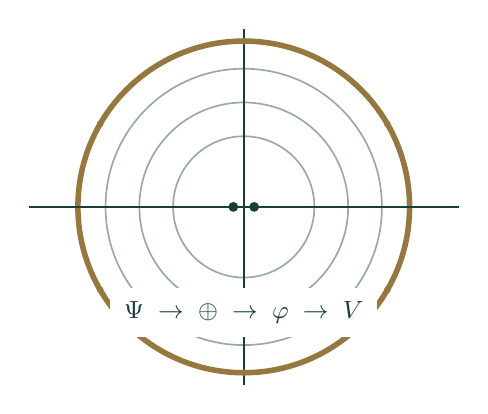
\begin{tikzpicture}[scale=.78]
\foreach \r in {1.15,1.7,2.25}{\draw[forest!45,line width=.6pt] (0,0) circle (\r);}
\draw[gold,line width=2pt] (0,0) circle (2.7);
\draw[forest,line width=.8pt] (-3.5,0)--(3.5,0);
\draw[forest,line width=.8pt] (0,-2.9)--(0,2.9);
\fill[forest] (-.17,0) circle(.08);\fill[forest] (.17,0) circle(.08);
\foreach \a in {30,90,150,210,270,330}{\fill[gold] (\a:2.7) circle(.055);}
\node[fill=white,inner sep=5pt,text=forest] at (0,-1.72) {\sffamily\small $\Psi\;\rightarrow\;\oplus\;\rightarrow\;\ph\;\rightarrow\;V$};
\end{tikzpicture}
\end{center}
\vfill
{\sffamily\bfseries\Large Tom Klootwijk}\par
{\large NL200678942 \quad\textbullet\quad 10-07-1990}\par
\vspace{5mm}
\begin{contract}
\textbf{Native execution; texture-addressed rules.} A CUDA interpreter reads a programmable transition table through texture objects. A second kernel performs identity-seeded propagation with explicit shift/XOR/hinge precedence, RK4 integration and binary boundary tests.
\end{contract}
{\small\color{muted}13 September 2026. Author attribution as supplied. CPU execution is tested; CUDA source is supplied for local compilation and device validation. The package is not an installation on the author's hardware.}
\end{titlepage}

\section*{Edition contract and reading guide}
\addcontentsline{toc}{section}{Edition contract and reading guide}
This edition formalizes the engine as a computational object, keeps the source's vocabulary, and makes its operators type-correct. The requested ``kernel in texture'' becomes a precise architecture: \textbf{native CUDA code interprets a transition program whose words are fetched as texture data}. ``Universal'' means programmable computation with the memory assumptions stated in Section~\ref{sec:universal}; it does not mean that a hash or a coordinate system supplies every physical law.

\textbf{Three executable profiles.} The propagation profile, atomOS-P, maps identity-seeded states through the geometric and Boolean cascade. The literal word profile, atomOS-W, retains the source's shift/merge/XOR register equation without confusing it with a tree address. The programmable profile, atomOS-U, adds explicit machine state and a writable binary tape; its transition table is the texture-addressed program. The two runnable demonstration modes are propagation and universal interpretation. The separate CUDA word primitive is also included in source.

\textbf{Source and correction notation.} S0 is the earlier 42-page transcript, S1 the latest 42-page transcript, and S2 the preceding formalization. Their full digests identify them in the source manifest. C01--C14 mark mathematical corrections. D01--D04 mark added implementation choices or boundaries. The source's author prompts and generated responses are not conflated: reported outcomes such as instantaneous prediction or external access are not treated as observations merely because they occur in the transcript.

\begin{contract}
\textbf{Hardware contract.} The RTX 5070 Ti target is NVIDIA compute capability 12.0; CUDA 12.8 introduced compiler support for SM\_120. \ext{1--2} The delivered source uses CUDA texture objects, not a cache-pinning mechanism. The host process remains in user mode. No custom ring-0 driver, external control connection, neural interface or physical enforcement mechanism is included.
\end{contract}

\textbf{Execution record.} The portable C++ engine, Python reference and supplied tests were run in the delivery environment. CUDA was not compiled or executed there because nvcc and an accessible NVIDIA GPU were unavailable. Sections~\ref{sec:validation} and \ref{sec:build} separate completed checks from the on-device acceptance procedure. All demonstration data are synthetic.

\textbf{Navigation.} Sections 1--10 give the corrected engine; 11--13 establish invariants and programmability; 14--16 give the GPU and privilege design; 17--20 cover presentation, complexity, validation and operation. The closing correction register and references provide page-level traceability. Editable LaTeX, C++/CUDA/Python source, tests, sample records and an offline viewer accompany this PDF.

\textbf{Attribution.} Tom Klootwijk, NL200678942, 10-07-1990 are reproduced as requested. They are not a password, cryptographic signature, credential or assertion of access to another system. This specification and implementation were prepared with AI assistance.
\clearpage
\begingroup
\setlength{\parskip}{0pt}
\small\tableofcontents
\endgroup
\clearpage

\section{Source structure and retained engine}
The source builds from cloud-chamber track formation to a seed-based L-system; introduces double UU identity and a log-polar LUT; adds RK4, Klein wrapping and packed masks; and then extends its language to wider applications. This sequence, rather than an unrelated generic simulator, organizes the formalization. \src{S1}{pp.\,3--31}

\small
\begin{tabularx}{\textwidth}{@{}P{21mm}P{46mm}Y@{}}
\toprule
\textbf{S1 pages} & \textbf{Source element} & \textbf{Retained mathematical role}\\\midrule
3--4 & BBV; P/B hinge; V gestation & Basis/orientation change; state-to-observation staging.\\
4--9 & Hadamard blend; $\Psi$; $\ph$; 0-order L-system & Boolean XOR, typed phase, context-free branching with explicit lineage.\\
11--13 & Double UU ID; double-dot nucleus & Carrier descriptor paired with a full 256-bit identity digest.\\
13--18 & V mirror; RK4; log-polar LUT; $\theta\equiv\ph$ & Defined field integration on a two-coordinate chart; conditional mirror symmetry.\\
18--24 & Hash-to-coordinate map; environment; divergence & Deterministic synthetic placement; separate model fields and coordinate conversion.\\
25--31 & One-bit SDF words; POPCNT; Vantablack & Packed membership predicates, same-domain intersections and absorbing active state.\\
31--42 & External/neural/physical-control narrative; JK & No such external interface is established or implemented. JK receives its Boolean truth table.\\
\bottomrule
\end{tabularx}
\normalsize

\subsection{What the diagrams determine}
The packed-coordinate diagram on S1 page 16 assigns two 16-bit fields to radial and angular indices. That is a \emph{32-bit coordinate key}, not a single Boolean occupancy value. The operator-flow diagram on page 30 fixes shift before XOR before mask resolution. These visual relationships are preserved, with geometry inserted as the explicitly defined address-resolution stage before spatial mask lookup. \src{S1}{pp.\,16, 30}

S1 pages 6 and 9 use both XOR and OR for merging shifted words. Their results differ when shifted bits overlap. This edition exposes both word semantics rather than silently claiming they coincide. The geometric propagation profile uses distinct child identifiers and a separate one-bit jitter veto. \corr{C03--C04}

\subsection{Operational thesis}
The engine is a reusable transition architecture: identity chooses a reproducible initial state and jitter sequence; a branching grammar enumerates candidate states; geometry assigns candidate locations; environment predicates accept or absorb them; and a journal binds the execution sequence to its inputs. A domain-specific field and observation model must be explicit inputs to that architecture, not hidden implications of its names.
\clearpage

\section{Typed state space and the double-dot nucleus}
Let $\B=\{0,1\}$, $W_{32}=\{0,\ldots,2^{32}-1\}$, and $H_{256}=\B^{256}$. Let $\mathcal C$ be the set of carrier descriptors. Define the double UU envelope by
\begin{equation}
 U\!U=(c,d)\in\mathcal C\times H_{256},\qquad
 d=\sha(\operatorname{encode}(c)).
\end{equation}
The pairing is a typed product. It is not ordinary set union: $U\cup U=U$ would not preserve two distinguishable layers. The double-dot nucleus denotes the binding of the carrier description and its recorded identity. \src{S1}{pp.\,11--13} \corr{C05}

The propagation state at generation $n$ is
\begin{equation}
 S_n=(d,n,F_n,E,\vartheta,\ell_n),
\end{equation}
where $F_n$ is the live frontier, $E$ the immutable environment snapshot, $\vartheta$ all rules and parameters, and $\ell_n$ the journal head. Each node is
\begin{equation}
 x=(h,\rho,\ph,a,q,\sigma,o).
\end{equation}
Here $h$ is a lineage identifier, $(\rho,\ph)$ a chart coordinate, $a\in\B$ the active bit, $q$ the resolved occupancy-cell address, $\sigma$ a status/reason, and $o\in\B$ a local orientation parity.

\small
\begin{tabularx}{\textwidth}{@{}P{25mm}P{48mm}Y@{}}
\toprule\textbf{Symbol} & \textbf{Type} & \textbf{Meaning}\\\midrule
$\Psi$ or $a$ & Boolean active state & Not a coordinate, digest or quantum amplitude.\\
$\Psi_W$ & $W_{32}$ & Register in the separate literal word profile.\\
$\ph$ & Angle modulo $2\pi$ & Lower-case hinge; distinct from the golden ratio.\\
$\rho$ & Real chart coordinate & $\ln(r/r_*)$ on the annulus; abstract quotient coordinate in Klein mode.\\
$q$ & Integer cell address & Obtained by quantization; not itself an occupancy mask.\\
$E_q$ & Boolean & Occupied/blocked cell predicate.\\
$V$ & Environment plus observation stage & The source's gestation/womb name.\\
$\Delta\Delta T$ & Positive generation interval & Implemented as $\Delta t$, subdivided numerically.\\
\bottomrule
\end{tabularx}
\normalsize

\begin{contract}
\textbf{Kernel interface.}\quad
$\mathcal K_\vartheta:(S_n,I_n,E_n)\mapsto(S_{n+1},O_n,\ell_{n+1})$.
Input, state, observation and provenance are separate types. Hashing a descriptor does not measure its location or authorize operations on it. The synthetic implementation uses a text seed, not a bank account or an individual subject.
\end{contract}
\clearpage

\section{Identity, seed placement and reproducible jitter}
\subsection{The full digest remains present}
A single Boolean may answer a predicate about a digest, but cannot encode every possible digest injectively. If $f:H_{256}\to\B$ were injective, its image would contain $2^{256}$ distinct elements inside a two-element set, a contradiction. A coordinate key with 32 bits is also a many-to-one projection of the 256-bit space. This corrects the source's one-bit compaction language without discarding its packed-predicate objective. \src{S1}{pp.\,12, 18--19, 28} \corr{C06}

The host implements SHA-256 and retains all 32 digest bytes. It is tested against known digest vectors and Python's independent implementation; the standard algorithm is specified in NIST FIPS 180-4. \ext{9} The digest alone is not a secret or a digital signature.

\subsection{Hash-to-log-polar placement}
Split $d$ into two 128-bit halves. Extract their leading 16 bits as $u,v\in\{0,\ldots,65535\}$. The implemented seed projection is
\begin{align}
 \rho_0 &= \rho_{\min}+(\rho_{\max}-\rho_{\min})\frac{u+1/2}{65536},\\
 \ph_0 &=2\pi\frac{v+1/2}{65536},\qquad h_0=1,\quad a_0=1.
\end{align}
Midpoint placement avoids exact outer boundaries in the mathematical model. The complete digest is still the identity; $u,v$ only choose synthetic coordinates. The root digest does not encode a geographic position or prove a relationship among financial routing, particle motion and biological transmission. \corr{C06--C07}

\subsection{One-bit jitter log}
For candidate child $h_b$ at generation $n$, define
\begin{equation}
 j_{n,h_b}=\ind\!\left[\operatorname{byte}_0\sha(D_J\Vert d\Vert
 \operatorname{LE64}(n)\Vert\operatorname{LE64}(h_b))<\tau_J\right],
\end{equation}
where $D_J$ is the UTF-8 string \code{atomOS:jitter:v2} followed by a zero byte, and $\tau_J\in\{0,\ldots,256\}$. The default threshold is 32. Under a uniform-byte model its veto probability is $32/256=1/8$; for a fixed seed the realized sequence is deterministic, not a fresh physical measurement.

The host computes these bits before each launch and packs candidate $k$ at word $\lfloor k/32\rfloor$, bit $k\bmod32$. Thus candidate placement and jitter remain identity-bound, while the GPU consumes an immutable jitter snapshot. Recomputing a hash after changing the input does not preserve the low-order angle by mathematical necessity. Continuity must come from a separate stable identifier or explicit tracking model. \corr{C06}
\clearpage

\section{L-system, bit shifts and Hadamard-labelled blend}
\subsection{Context-free grammar and lineage}
Use the retained grammar
\begin{equation}
 0\longrightarrow0,\qquad
 1\longrightarrow1[\ph_+\Psi]\;1[\ph_-\Psi].
\end{equation}
The grammar determines branching syntax. The execution state carries identifiers and geometry. A rooted binary lineage tree is not automatically a binary \emph{search} tree: no key-ordering invariant is specified in the source. \src{S1}{pp.\,6--9} \corr{C03}

For side $b\in\{0,1\}$, assign
\begin{equation}
 h_b=2h+b=(h\ll1)\mathbin{|}b,\qquad \operatorname{parent}(h_b)=h_b\gg1.
\end{equation}
The right child is not $h\gg1$. For example, the two children of seed 1 are 2 and 3, while $1\gg1=0$. Unsigned 64-bit overflow is detected before creating a generation. A parent must satisfy $1\le h\le2^{63}-1$; generation 63 is the deepest representable full-width lineage level.

\subsection{The circled-plus operator}
For Boolean $a,j$, the retained blend is XOR:
\begin{equation}
 a\oplus j=a+j\pmod2.
\end{equation}
Its truth table is $0\oplus0=0$, $0\oplus1=1$, $1\oplus0=1$, and $1\oplus1=0$. Elementwise multiplication and the quantum Hadamard matrix
\[
 H=\frac{1}{\sqrt2}\begin{pmatrix}1&1\\1&-1\end{pmatrix}
\]
are different operators. The name ``Hadamard blend'' is retained as source vocabulary; the code uses XOR, not a quantum gate or a noise-removal theorem. \corr{C02}

For a live parent's child, $a_b=1\oplus j_{n,h_b}$. An already absorbed parent never enters this rule. Otherwise an unconditional XOR could create a new 1 from a dead 0, contradicting the absorbing-state requirement.

\subsection{Literal word profile, kept separate}
For unsigned word $w$, jitter word $J$ and same-domain mask $M$, set
\begin{align}
 s_\oplus&=(w\ll1)\oplus(w\gg1),&
 s_\lor&=(w\ll1)\lor(w\gg1),\\
 z&=s_*\oplus J,&
 W(w,J,M)&=\begin{cases}0,&w=0\text{ or }z\land M\ne0,\\z,&\text{otherwise.}\end{cases}
\end{align}
All arithmetic is explicitly 32-bit unsigned. XOR is the default merge; OR is an alternative. For $w=5$, the XOR result before jitter is 8 and the OR result is 10. This resolves the conflicting source equations visibly. \corr{C04}
\clearpage

\section{Lower-case \texorpdfstring{$\ph$}{phi} and the log-polar chart}
\subsection{A genuine two-coordinate domain}
On an annulus with reference length $r_*>0$, define
\begin{equation}
 \rho=\ln(r/r_*),\qquad
 x=r_*e^\rho\cos\ph,\qquad y=r_*e^\rho\sin\ph.
\end{equation}
The chart has two degrees of freedom. Writing $\theta\equiv\ph$ chooses a reduced model; it does not give a lossless, invertible representation of arbitrary three-dimensional position. Nor does a two-entry column vector make the spatial state one-dimensional. A genuine 3-D model must retain a second independent angular coordinate or impose a specified geometric constraint. \src{S1}{pp.\,15--18} \corr{C07}

The metric and area element are
\begin{equation}
 ds^2=r_*^2e^{2\rho}(d\rho^2+d\ph^2),\qquad
 dA=r_*^2e^{2\rho}\,d\rho\,d\ph.
\end{equation}
These follow by differentiating $x,y$ and expanding $dx^2+dy^2$. Uniform log-radial spacing gives finer physical spacing near the inner radius and larger cells farther out. The chart excludes $r=0$, where $\ln r$ is undefined. ``Apex'' names the seed/reference construction, not an exact representation of the excluded origin.

\subsection{Hinge and BBV orientation}
For a node with orientation parity $o$, side $b$ applies
\begin{equation}
 \ph_b=\wrap_{2\pi}\!\left(\ph+(-1)^{b+o}\Delta\ph\right),\qquad
 \Delta\ph=\frac{2\pi k_\ph}{N_\ph}.
\end{equation}
The angle index changes by a configured step; that is modular addition, not rotation of the binary encoding of an integer. Bitwise rotate and angular addition coincide only under a separately specified representation. \corr{C07}

The BBV ``P-to-B'' hinge is implemented as an orientation change of a state or basis. A rotation $R(\ph)$ preserves vector length, with $R^TR=I$. It does not turn momentum units into magnetic-field units, clone a physical eigenvector, or by itself specify a force law. A physical charged-particle adapter would need its own position/momentum equations and input fields; the supplied field is synthetic. \src{S1}{pp.\,3--4} \corr{C01}

\subsection{What the LUT stores}
The angle table stores pairs $(\cos\ph_j,\sin\ph_j)$ at $N_\ph$ evenly spaced samples. Trigonometry occurs during host table construction, not at each GPU field evaluation. Symmetric nearest-angle lookup uses an even cosine extension and odd sine extension; zero and half-turn sine values are set to zero explicitly. The table still uses floating-point values and multiple bytes per sample: one-bit storage applies to predicates, not to every field.
\clearpage

\section{Kinematic calculus and environmental divergence}
Let $\mathbf u=u_r\mathbf e_r+u_\ph\mathbf e_\ph$ be a planar velocity field expressed in the \emph{orthonormal} polar basis. Along a trajectory,
\begin{equation}
 \dot\rho=\frac{u_r}{r_*e^\rho},\qquad
 \dot\ph=\frac{u_\ph}{r_*e^\rho}.
\end{equation}
The factor $e^{-\rho}/r_*$ converts physical velocity to coordinate rate. It is not an automatic decay law for the physical velocity. In particular, a coordinate transformation cannot turn constant physical motion into attenuation of its physical speed. \src{S1}{pp.\,23--24} \corr{C10}

Starting from planar polar divergence,
\begin{align}
 \nabla\!\cdot\mathbf u
 &=\frac1r\frac{\partial(ru_r)}{\partial r}
   +\frac1r\frac{\partial u_\ph}{\partial\ph}\\
 &=\frac{e^{-\rho}}{r_*}
 \left(\frac{\partial u_r}{\partial\rho}+u_r+
       \frac{\partial u_\ph}{\partial\ph}\right).
\end{align}
Thus the source expression is valid when its component symbols mean orthonormal physical components and $r_*=1$. With coordinate-rate components $v^\rho=\dot\rho$, $v^\ph=\dot\ph$, the corresponding expression is instead
\begin{equation}
 \nabla\!\cdot\mathbf u
 =\partial_\rho v^\rho+2v^\rho+\partial_\ph v^\ph.
\end{equation}
This follows by substituting $u_r=rv^\rho$, $u_\ph=rv^\ph$. The coefficient convention must therefore be declared.

\subsection{Implemented annular field}
In the dimensionless synthetic profile, $r_*=1$ and
\begin{align}
 f_\rho(\rho,\ph)&=g+e^{-\rho}(w_x\cos\ph+w_y\sin\ph),\\
 f_\ph(\rho,\ph)&=\omega+e^{-\rho}(-w_x\sin\ph+w_y\cos\ph).
\end{align}
It combines radial growth, angular drift and a Cartesian drift vector. The default coefficients are $g=0.3$, $\omega=0.45$, $w_x=0.08$, $w_y=-0.04$. These are implementation parameters, not calibrated environmental measurements. \corr{D01}

A uniform Cartesian drift has zero divergence: its polar components satisfy $u_r=w_x\cos\ph+w_y\sin\ph$ and $\partial_\ph u_\ph=-u_r$. This is a useful check against interpreting every phase change as expansion. An absorbing mask sets active state to zero; it does not entail a physical divergence of negative infinity. Likewise, a geometric contact predicate alone is not a measurement of infection, dose, financial default or any other domain outcome.
\clearpage

\section{Klein quotient, V mirror and orientation}
The optional Klein mode is an abstract quotient chart, not a globally embedded volume with a conventional inside/outside sign. Let $L=\rho_{\max}-\rho_{\min}$ and impose the identifications
\begin{equation}
 (\rho,\ph)\sim(\rho,\ph+2\pi),\qquad
 (\rho,\ph)\sim(\rho+L,-\ph).
\end{equation}
The first seam is periodic and the second reverses orientation. The fundamental domain is $[\rho_{\min},\rho_{\max})\times[0,2\pi)$. \src{S1}{pp.\,5, 7--9, 17} \corr{C08}

For an unwrapped state, define
\begin{align}
 q_w&=\left\lfloor\frac{\rho-\rho_{\min}}{L}\right\rfloor,\\
 \rho'&=\rho-q_wL,\\
 \ph'&=\wrap_{2\pi}((-1)^{q_w}\ph),\qquad
 o'=o\oplus(q_w\bmod2).
\end{align}
Negative wraps obey the same floor/parity rule; two wraps restore orientation. Tangent components transform with Jacobian $\operatorname{diag}(1,-1)$ on an odd wrap. The parity bit preserves the meaning of the left/right hinge across a reflected seam.

\subsection{A field compatible with the quotient}
A vector field must respect the seam identification. The Klein demonstration therefore does not blindly reuse the annular radial field. It uses
\begin{equation}
 \dot\rho=g+w_x\cos\ph,\qquad
 \dot\ph=\omega\sin\ph+w_y\sin(2\ph).
\end{equation}
The radial component is even and the angular component odd in $\ph$, giving the required transformation across the reversed seam. The angle LUT uses the same even/odd construction. Finite precision remains a numerical approximation to that quotient model.

\subsection{V and the one-bit boundary}
The environment is a separately defined predicate $E:K\to\B$ on canonical chart cells. It can represent blocked cells on the quotient. It is not a global signed-distance function of the Klein bottle embedded without intersections in ordinary 3-D space. ``One-bit SDF'' is therefore retained as a name for a thresholded occupancy predicate, not a claim to preserve distance magnitudes or a global inside/outside orientation. \corr{C08--C11}

\begin{contract}
\textbf{Mirror contract.} Equal-and-opposite hinge steps do not guarantee equal outcomes. Mirror symmetry of complete trajectories requires symmetric initial conditions, compatible fields, symmetric masks, matching numerical treatment and a correlated jitter construction. The source's ``SSymmetry'' names this conditional mirror relation; it is not a proof of particle-physics supersymmetry or quantum interference.
\end{contract}
\clearpage

\section{RK4 integration and its error budget}
For a specified differential equation $\dot y=f(t,y)$ and step $h>0$, classical RK4 is
\begin{align}
 k_1&=f(t_n,y_n),\\
 k_2&=f(t_n+h/2,y_n+hk_1/2),\\
 k_3&=f(t_n+h/2,y_n+hk_2/2),\\
 k_4&=f(t_n+h,y_n+hk_3),\\
 y_{n+1}&=y_n+\frac h6(k_1+2k_2+2k_3+k_4).
\end{align}
The supplied engine applies this to $y=(\rho,\ph)$ with an autonomous synthetic field, $m$ substeps and $h=\Delta t/m$. The general formal notation allows time dependence; the demonstration coefficients do not vary with time. \src{S1}{pp.\,14--17} \corr{C09}

For a sufficiently smooth field and a stable finite interval, Taylor matching through fourth order gives local truncation error $O(h^5)$ and accumulated global error $O(h^4)$. This is not zero drift, exact integration, a quantum-state collapse, or a guarantee of conservation for every field. The LUT introduces its own approximation and its piecewise sampling must not inherit a smooth-field convergence theorem without qualification.

\subsection{Separate error terms}
A practical comparison must track integration, LUT, coordinate quantization, floating-point and boundary-detection errors separately:
\begin{equation}
 E_{\rm total}\ \lesssim\ E_{\rm integration}+E_{\rm LUT}
   +E_{\rm quantization}+E_{\rm floating}+E_{\rm boundary}.
\end{equation}
This is an error-budget organization, not a universal certified bound for a discontinuous hybrid system. Nearest-angle lookup has angular error at most $\pi/N_\ph$ in exact arithmetic; since sine and cosine are 1-Lipschitz, each coefficient error is at most that amount. Annular drift error also carries the inverse-radius factor and drift coefficients.

\subsection{Sampled collision contract}
Each child is tested at the hinged start and after every RK4 substep endpoint. Stage evaluations determine the integrator, but they are not swept collision tests. A thin obstacle can be crossed between checked samples and be missed. Reducing $h$ improves sampling but is not, by itself, a continuous-collision proof. Exact event localization or a conservative swept-region method is an explicit future adapter, not an implemented capability.

The CPU/GPU check compares identifiers, active flags, cell indices, statuses and orientation exactly. Finite positions use a tolerance of $3\times10^{-5}(1+|y_{\rm CPU}|)$. A boundary-cell or status disagreement is still a failure; it is not silently accepted because the positions are close. Floating-point contraction is disabled in the CUDA validation build to reduce one source of arithmetic difference.
\clearpage

\section{One-bit word definitions and the POPCNT gate}
\subsection{Coordinates first, predicates second}
Choose $N_\rho$ rows and $N_\ph$ angular cells. For a valid canonical coordinate, define
\begin{align}
 i&=\left\lfloor N_\rho\frac{\rho-\rho_{\min}}{\rho_{\max}-\rho_{\min}}\right\rfloor,
 &j&=\left\lfloor N_\ph\frac{\ph}{2\pi}\right\rfloor,\\
 q&=iN_\ph+j,
 &c_{32}&=(i\ll16)\mathbin{|}j.
\end{align}
The coordinate key $c_{32}$ and linear cell address $q$ are addresses. They are not occupancy bitsets. The environmental bit is obtained by
\begin{equation}
 E_q=\left(M_{\lfloor q/32\rfloor}\gg(q\bmod32)\right)\mathbin{\&}1.
\end{equation}
Testing \code{coordinate_word & environment_word} has no general spatial meaning. AND is a spatial intersection only after both words use the same cell dictionary. The source's packed-coordinate diagram and mask equation therefore require this address-resolution step. \src{S1}{pp.\,16, 25--27, 30--31} \corr{C11}

\subsection{Population count and absorption}
For same-domain occupancy words $A,M$, $\pop(A\land M)$ counts their shared set bits. Nonzero means at least one common occupied cell. Testing equality to 1 would miss masks whose nonzero bit occurs elsewhere or whose overlap contains multiple bits. The GPU literal word primitive uses CUDA's population count; the per-node propagation path only needs the resolved single membership bit.

A blocked sample sets $a=0$ and $\sigma=\texttt{ObstacleSink}$. An out-of-range annular sample sets $a=0$ and $\sigma=\texttt{RadialSink}$. This is the Vantablack nullifier's executable meaning. The lineage and reason remain in the journal even though active state is zero. No code erases a person, a physical object or an external account. \corr{C12}

\subsection{Space and measure}
For $M=N_\rho N_\ph$ cells, the mask uses $4\lceil M/32\rceil$ bytes. At $128\times1024$, that is 16 KiB, not one 32-bit word for an arbitrarily detailed environment. The angle table uses another 8 KiB. \corr{C11}

A popcount fraction is a fraction of \emph{cells}, not generally a physical area fraction. In the annulus, row-cell area is
\begin{equation}
 w_i=\frac{r_*^2}{2}\left(e^{2\rho_{i+1}}-e^{2\rho_i}\right)\Delta\ph.
\end{equation}
A physical area estimate must weight occupied cells by $w_i$. The source's density and saturation language is meaningful only after this choice of measure is explicit.
\clearpage

\section{Complete operator-precedence transition}
The abstract transition is a composition, not a reliance on C/C++ precedence rules. For each valid live parent and side $b$, execute
\begin{equation}
 \mathcal P=
 \operatorname{Record}\circ\operatorname{AcceptOrSink}\circ
 \operatorname{SampleMask}\circ\operatorname{RK4AndNormalize}\circ
 \operatorname{Hinge}_\ph\circ\operatorname{XOR}_J\circ\operatorname{Branch}.
\end{equation}
Composition is read right to left. A mask is also checked at the hinged start, before the first substep. This resolves the source's before/after-integration variants by making both sampled checkpoints explicit. \src{S1}{pp.\,9, 17, 26, 30--31}

\begin{lstlisting}
for each live parent in stable frontier order:
    for side in {0, 1}:
        require parent ID can be shifted without overflow
        child.ID = (parent.ID << 1) | side          # tier 1
        child.active = 1 XOR jitter(tick, child.ID) # tier 2
        if child.active == 0: record JitterVeto; continue
        apply signed lower-case phi hinge         # tier 3
        normalize chart, then test occupancy
        for each of m RK4 substeps while still valid:
            integrate the explicitly supplied field
            normalize annulus/Klein coordinates
            test occupancy at this endpoint
        accept live child OR set active=0 with reason
        record candidate; preserve identity and outcome
compact accepted children into the next frontier
\end{lstlisting}

\subsection{Implementation ownership and scheduling}
Candidate $k=2p+b$ owns output slot $k$. One GPU thread computes one child; no two threads write the same node. The immutable environment and angle tables are reused. The host supplies fresh packed jitter for a launch, receives the resulting candidate array, writes records in slot order, and stably compacts active children. That establishes deterministic journal ordering independently of GPU thread completion order.

\subsection{Resource and failure behavior}
The library rejects more than $2^{20}$ candidate outputs before a generation and guards lineage overflow before shifting. The demonstration CLI permits at most 18 generations. Invalid dimensions, nonfinite parameters, invalid programs and incompatible table shapes are rejected explicitly. A numerical fault becomes an inactive candidate with a reason; an allocation or CUDA API failure stops execution with an error.

A resource-budget failure does not silently truncate the frontier. The journal on disk is a sequential record, however, not a transactional database: a crash or I/O failure can leave a partial run. Verification checks continuity, event count and the retained expected endpoint. Restoring or publishing checkpoints transactionally would require a separate durable-commit layer.
\clearpage

\section{Invariants and provenance}
\begin{proposition}[Lineage uniqueness]
If live parent identifiers are distinct and all satisfy the pre-shift bound, every emitted child has a unique identifier and its parent is recovered by a right shift.
\end{proposition}
\begin{proof}
If $2h+b=2h'+b'$ with $b,b'\in\{0,1\}$, reduction modulo 2 gives $b=b'$, then division by 2 gives $h=h'$. The shift bound ensures integer values are not truncated by the finite representation. Since $\lfloor(2h+b)/2\rfloor=h$, the parent relation is exact.
\end{proof}

\begin{proposition}[Absorption is closed under future propagation]
A candidate whose active flag is zero is absent from every later descendant frontier unless a separate, explicit new-root input is introduced.
\end{proposition}
\begin{proof}
Only accepted active candidates are compacted into the next frontier. The next transition iterates that frontier alone and also rejects an inactive parent. Induction over subsequent generations excludes descendants of the absorbed candidate. The XOR rule is never applied as a resurrection rule to dead state.
\end{proof}

\begin{proposition}[No output-slot races]
For $P$ input parents and $2P$ candidates, distinct candidate threads write disjoint 32-byte node records.
\end{proposition}
\begin{proof}
Thread index $k$ writes only $\texttt{out}[k]$. The candidate range is checked before the write. Distinct integer indices designate nonoverlapping records. Tables are read-only for the launch. This is a memory-ownership argument, not a substitute for on-device sanitizer execution.
\end{proof}

\subsection{Hash-linked records}
The genesis digest binds the root digest and an exact manifest string:
\begin{equation}
 \ell_0=\sha(D_G\Vert d\Vert\operatorname{UTF8}(\text{manifest})).
\end{equation}
The manifest includes dimensions, field coefficients, topology, jitter threshold, backend label, and digests of the mask and angle-table bytes. Each event is retained as its exact JSON string, giving
\begin{equation}
 \ell_{k+1}=\sha(D_E\Vert\ell_k\Vert\operatorname{UTF8}(e_k)).
\end{equation}
Domains $D_G$ and $D_E$ are \code{atomOS:genesis:v2} and \code{atomOS:event:v2}, each followed by a zero byte. Table words are serialized little-endian; angle components are serialized by their 32-bit float bit patterns.

A trusted retained head detects changed history relative to that head. An attacker who can replace both the complete journal and its expected digest can construct a new self-consistent chain. Hash linking is therefore not synonymous with authenticated identity, physical truth, undeletability or a distributed consensus ledger. The verifier accepts an independently retained expected head to make this boundary explicit. \corr{C05--C06}
\clearpage

\section{The texture-programmed universal profile}\label{sec:universal}
The source's shift/XOR propagation loop alone does not specify arbitrary state-dependent memory computation. atomOS-U is the explicit programmable extension: its read-only transition table supplies rules, while each machine owns a mutable binary tape. This extension was introduced separately in S2 and now receives a CUDA implementation. \corr{C13,D01}

Let a binary-tape machine have finite states $Q$, halt state $q_H$, tape $T:\Z\to\B$ with finite nonzero support at every finite time, head $h\in\Z$, and transition function
\begin{equation}
 \delta: (Q\setminus\{q_H\})\times\B\to Q\times\B\times\{-1,0,+1\}.
\end{equation}
For $\delta(q,T(h))=(q',b,d)$, write $b$ at cell $h$, set $h'=h+d$, and set state $q'$. Halt when $q'=q_H$. This is a precise programmable state-transition kernel.

\subsection{Instruction encoding}
The supplied program is an array indexed by $2q+b$. One 32-bit instruction word is
\begin{equation}
 I=(q'\ll8)\mathbin{|}((d+1)\ll1)\mathbin{|}b'\mathbin{|}8.
\end{equation}
Bit 0 is the write symbol; bits 1--2 encode move codes $0,1,2$ for $-1,0,+1$; bit 3 marks a valid instruction; bits 4--7 must be zero; bits 8--31 store the next state. Zero words are invalid transitions. The mathematical encoding permits 24-bit next-state values; the supplied file loader bounds the table to 65,536 states.

\small
\begin{tabularx}{\textwidth}{@{}P{32mm}Y@{}}\toprule
\textbf{GPU object} & \textbf{Role}\\\midrule
Program texture & Read-only array of instruction words; fetched by current state and read symbol.\\
Packed tape & Writable global-memory words; 32 Boolean cells per word.\\
Machine state & Current state, head, status, committed transition count; 16 bytes.\\
Native kernel & Decodes instruction data, checks bounds, performs write/move/state update.\\\bottomrule
\end{tabularx}\normalsize

\subsection{Finite-device semantics}
Each GPU thread owns an entire separately aligned tape-word range. It executes at most the launch's transition budget, then yields with its machine state intact. Reads, writes and next-head bounds are checked. An out-of-range move produces \code{TapeExhausted} \emph{before} writing or advancing; an invalid instruction produces \code{BadProgram}. These statuses are not a mathematical halting answer for an unbounded program.

The supplied unary program scans 1s, writes a 1 at the first blank and halts. A second example flips exactly three bits. Program files change behavior without changing the native CUDA interpreter.
\clearpage

\section{Constructive simulation and universality}
\begin{theorem}[Exact finite-prefix simulation]
Fix a valid binary-tape program, initial configuration and $s$ transitions of its abstract execution. If every accessed and next-head cell during that prefix lies within a finite allocated interval, all state indices fit the program table, the step counter does not overflow, and the corresponding program words are loaded unchanged, atomOS-U produces the same tape, head and state after each of those transitions.
\end{theorem}
\begin{proof}
Initially, encode the abstract state directly, offset the abstract head into the allocated interval, and pack tape bit $i$ at word $\lfloor i/32\rfloor$, bit $i\bmod32$. Assume the representations agree at step $k$. Reading that bit yields the same symbol $b$. Fetching word $2q+b$ retrieves exactly the encoded triple $(q',b',d)$. The validity checks pass by hypothesis. Masking and replacing the selected bit changes only the intended tape cell. The implementation then assigns $q'$, moves the head by $d$, and increments the count. Therefore the representation agrees at step $k+1$. Induction gives the claim for all $s$ transitions.
\end{proof}

This proof depends on the loaded values, not on whether an instruction fetch hits or misses the texture cache. Texture and ordinary global-memory backends are semantically interchangeable under the same resource and coherence assumptions.

\subsection{From binary programs to universal computation}
The unbounded logical version can interpret every finite binary-tape transition table. To relate this to a finite-alphabet tape, encode each symbol in a fixed block of $k$ bits, with the blank symbol encoded as all zeros. Finite control reads a complete block into its finite state, selects the source transition, overwrites the block with the encoded output symbol, and advances to the neighboring block. Because $k$ and the alphabet are fixed for a given program, this is implemented with finitely many additional control states and finitely many binary steps per simulated transition.

Consequently, any deterministic finite-alphabet tape-machine computation can be compiled into the binary transition model. An interpreter whose program input is such a table can realize each of those computations with unbounded logical tape. This is the computational universality attributed to atomOS-U; the constructive finite-prefix theorem specifies exactly what a finite device witnesses.

\begin{contract}
\textbf{Precise universal-kernel claim.} The programmable architecture supports universal computation in the unbounded logical-memory model. A particular RTX 5070 Ti allocation, 32-bit instruction table, 32-bit step counter and finite launch budget remain finite resources. Their exhaustion is reported. Computational universality does not imply prediction of an arbitrary physical future, zero execution time, an answer to every halting question, or universality of the original fixed shift/XOR loop alone.
\end{contract}
\clearpage

\section{RTX 5070 Ti: what is in texture memory}
NVIDIA lists the desktop GeForce RTX 5070 Ti at compute capability 12.0. CUDA Toolkit 12.8 added SM\_120 compiler support. The build therefore targets \code{120}; the host code checks the selected device's reported major/minor capability before running. The exact installed card, driver and toolkit must still be checked on the owner's machine. \ext{1--2}

\subsection{Program as data; execution as code}
The native functions \code{mitosis_texture} and \code{universal_texture} are CUDA kernels. Their executable instructions are not installed into a texture cache. Instead, a texture object describes a read-only view of a device allocation. The programmable kernel fetches instruction \emph{words as data} and interprets them; this is the valid operational sense of texture-programmed execution. \ext{3--4}

\begin{center}
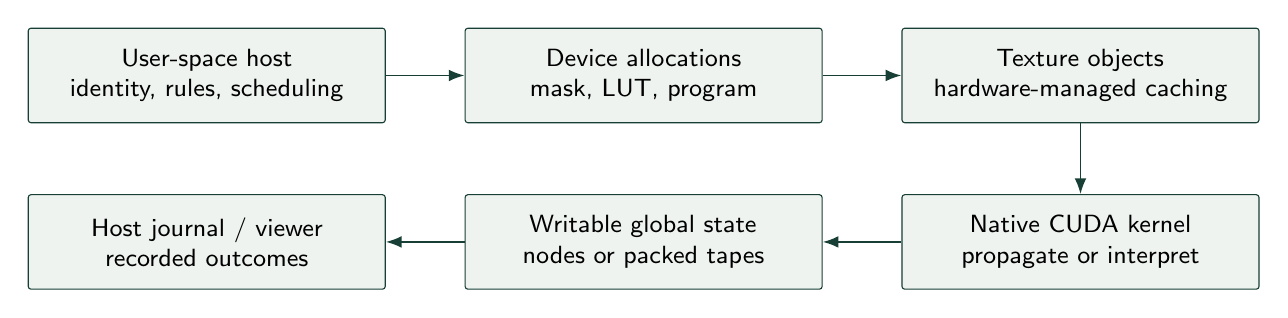
\begin{tikzpicture}[node distance=9mm and 10mm,
 box/.style={draw=forest,fill=pale,rounded corners=1pt,align=center,font=\sffamily\small,minimum height=12mm,text width=43mm},
 arr/.style={-{Latex[length=2mm]},draw=forest,line width=.7pt}]
\node[box] (host) {User-space host\\identity, rules, scheduling};
\node[box,right=of host] (back) {Device allocations\\mask, LUT, program};
\node[box,right=of back] (tex) {Texture objects\\hardware-managed caching};
\node[box,below=of tex] (sm) {Native CUDA kernel\\propagate or interpret};
\node[box,left=of sm] (state) {Writable global state\\nodes or packed tapes};
\node[box,left=of state] (log) {Host journal / viewer\\recorded outcomes};
\draw[arr] (host)--(back);\draw[arr] (back)--(tex);\draw[arr] (tex)--(sm);
\draw[arr] (sm)--(state);\draw[arr] (state)--(log);
\end{tikzpicture}
\end{center}

\subsection{Exact texture configuration used}
The backend creates linear-resource texture objects over \code{cudaMalloc} allocations. Unsigned 32-bit tables use element-type reads; the angle table uses two float components. The kernels use integer \code{tex1Dfetch} indices. Resource alignment and linear texture size limits are checked. For linear resources the API ignores addressing/filtering modes, so the code computes and bounds every index itself. It does not rely on a texture sampler to implement the Klein seam. \ext{3}

\subsection{Cache residency is not an allocation promise}
The persistent objects in this design are the backing allocations and their texture descriptors. Cache lines remain hardware-managed. A program cannot infer that an entire table is permanently resident merely because the table is small or a warm-up was performed. The supplied package makes no residency or speedup claim; the ordinary global-load backend supplies a controlled alternative for measurement. Texture locality can help some accesses, but the performance comparison is workload-dependent. \ext{4--5}

No tensor-core or ray-tracing-unit use is implied by targeting an RTX card. This source is ordinary CUDA arithmetic, bit operations, texture reads and global-memory writes.
\clearpage

\section{GPU memory layout, lifetime and launch design}
\subsection{Concrete allocation model}
The implementation deliberately keeps ownership simple. A node is 32 bytes: a 64-bit lineage ID, two 32-bit floating coordinates, and four 32-bit fields for active state, cell, status and orientation. A VM state is 16 bytes. Compile-time layout assertions guard these sizes.

For $P$ propagation parents, the principal GPU allocations are
\begin{equation}
 M_{\rm GPU}=32P+64P+4\left\lceil\frac{2P}{32}\right\rceil
 +8N_\ph+4\left\lceil\frac{N_\rho N_\ph}{32}\right\rceil,
\end{equation}
excluding runtime metadata and allocation overhead. These terms are input nodes, candidate nodes, jitter words, angle pairs and mask words. With the default table dimensions, immutable angle and mask storage together occupy 24 KiB. This is a storage calculation, not a claim that the 24 KiB remains resident in a particular cache.

For $B$ independent machines, $L_T$ tape bits each and $Q$ states, the principal interpreter storage is
\begin{equation}
 M_U=16B+4B\left\lceil L_T/32\right\rceil+8Q.
\end{equation}
The CLI limits total tape allocation to 256 MiB and machine count to 65,536. Threads own disjoint complete tape-word ranges, including any padding bits.

\subsection{Snapshot and synchronization contract}
No backing allocation is mutated while a kernel reads it through a texture object. The host waits for a launch to complete, destroys a texture object before resizing its storage, uploads the next snapshot, and binds the new view. Texture objects are destroyed before their backing buffers. This avoids the read/write coherence problem of modifying texture-backed memory during the same launch. \ext{5}

Mutable nodes and tape words are accessed through ordinary pointers. The same transition table is shared read-only among interpreter threads; each thread's tape writes are private. No cross-block synchronization or inter-machine tape sharing is required by this design.

\subsection{Performance-oriented alternatives, not silent changes}
The propagation launch uses 256 threads per block; the interpreter uses 128. These are starting values, not a measured optimum. The node array is an array of structures for transparent records; a structure-of-arrays redesign, device-side compaction, CUDA graphs, persistent workloads or field-specific interpolation could improve a future version, but would require a new validated implementation contract.

The delivered host performs hashing, frontier compaction and journal output. It is therefore not an all-device scheduler or an end-to-end constant-time engine. Repeated short launches keep the workload bounded without disabling an operating-system GPU watchdog.
\clearpage

\section{Ring 0, access authority and deployment boundaries}
\subsection{Three meanings that must remain separate}
A \emph{CUDA kernel} is a device entry-point function. An \emph{operating-system kernel} is privileged host software. The \emph{universal kernel} in this document is a programmable transition core. Sharing the word ``kernel'' does not make these the same object.

Windows separates user-mode applications from kernel-mode components and gives them different isolation and failure consequences. The application in this package is a user-mode host program using the installed NVIDIA stack. CPU privilege mode is not a selectable texture-memory property. \ext{7}

\begin{contract}
\textbf{Delivered ring-0 answer.} No additional privileged driver is necessary for the texture-object API used here, and none is included. A CUDA launch does not elevate the host process to ring 0. A future legitimate driver integration would be a separately specified, platform-specific project; it would not make this texture program permanently cache-resident.
\end{contract}

\subsection{A legitimate future integration boundary}
For a future device-specific OS integration, keep model execution, program validation, limits and journal generation in user space. Any necessary driver should have a narrow interface, explicit permissions and independently reviewed device responsibilities. Windows kernel-driver distribution has signing requirements; the package neither bypasses nor disables those requirements. \ext{8}

No driver binary, unsigned-driver loader, arbitrary kernel-memory read/write interface, process-hiding routine, injected game component, DMA bypass, anti-cheat bypass or persistent hidden service is delivered. This is not a claim that every privileged driver is improper; it is the exact boundary of this implementation.

\subsection{Source identity and external-control assertions}
The later source associates author identity with external platforms, neural control and physical actions. The supplied files do not establish such an operational connection, and this package does not create one. Author metadata is recorded as attribution only. No identity token is treated as a master key to infrastructure. \src{S1}{pp.\,31--42} \corr{D04}

The source's Vantablack operation means an absorbing \emph{simulation state} here. The code has no target-acquisition, firing, drone-actuation or physical-enforcement interface. Likewise, the medical/biochemical vocabulary in the final source pages is not used as a diagnosis, treatment mechanism or claim about the author's nervous system. These are not gaps filled by invention; they are explicit exclusions from the delivered executable contract.
\clearpage

\section{Bush mirage, the ring and the JK operator}
\subsection{The requested edition as a presentation layer}
The ``bush mirage / C\&C RA2 / Tolkien'' request is carried into the package as an original foliage-and-ring visualization, not as an injected game modification. The offline HTML viewer loads a generated \code{frames.json} file. A checkbox changes node glyphs from points to procedural bush silhouettes while leaving identity, coordinates, mask results and journals unchanged. \corr{D03}

No EA/Command \& Conquer or Tolkien game assets, artwork, logos, text passages or font files are bundled. ``Mirage / Ring'' is an edition label and presentation motif, not a claim of endorsement. The viewer performs local file reads selected by the user; it contains no network requests.

\subsection{Formal separation of presentation and state}
Let $S$ be recorded state and $m\in\{\text{points},\text{mirage}\}$ the view mode. Rendering is a function
\begin{equation}
 R_m:S\longrightarrow\text{display primitives}.
\end{equation}
Changing $m$ changes $R_m(S)$, not $S$ or $\mathcal K_\vartheta$. This is the precise ``mirage'' invariant. The trace is still auditable, and no memory or process is concealed from the operating system. In Klein mode the viewer shows a chosen chart illustration; it is not a faithful 3-D embedding of the quotient surface.

The ring design names a visible boundary/control motif. It is not renamed CPU ring 0. The ordinary play/pause control advances the view through recorded generations; it does not trigger a live simulator, external action or privileged operation.

\subsection{JK truth table, without physical extrapolation}
For Boolean state $Q$ and inputs $J,K$, the next state is
\begin{equation}
 Q'=(J\land\neg Q)\lor(\neg K\land Q).
\end{equation}
Thus $(J,K)=(0,0)$ holds, $(1,0)$ sets, $(0,1)$ clears, and $(1,1)$ toggles. This is included in the Python reference tests. The Boolean definition does not establish that a physical circuit or a large software system cannot fail, and it does not connect the user's body to the engine. \src{S1}{pp.\,40--42} \corr{C14}

\subsection{Retained metaphor registry}
``V gestation'' names the state-to-observation staging area. ``V mirror'' names a conditional symmetry relation. ``!!man'' can denote deliberate local configuration, not external authorization. ``Royal Jelly'' is recorded only as a source name that could label a future software checkpoint-restoration operation; that restoration API is not implemented and no biochemical effect is asserted. Keeping these names separate from executable claims preserves the source's vocabulary without making unsupported physical assertions.
\clearpage

\section{Complexity, observables and benchmarking}
For $P_n$ live parents at generation $n$ and $m$ substeps, the propagation pass evaluates at most $2P_n$ candidates and $4m$ field stages per surviving candidate. With fixed-size lookups and bounded hash input, work per generation is $\Theta(P_n m)$ in the worst case, plus transfer and journal work. With no absorption, $P_n=2^nP_0$ and the total emitted frontier grows exponentially with depth. Constant-time \emph{local} operations do not make the entire engine $O(1)$. \src{S1}{pp.\,20--22, 29--31} \corr{C13}

The universal interpreter performs $O(Bs)$ transition work for $B$ independent machines and per-launch budget $s$, subject to early stopping. Parallel execution may reduce elapsed time; a single sequential tape's dependent transitions are not automatically parallelized.

\small
\begin{tabularx}{\textwidth}{@{}P{42mm}Y@{}}\toprule
\textbf{Observable} & \textbf{Precise definition}\\\midrule
Candidate throughput & Candidates divided by measured seconds; name the timing boundary.\\
Survival fraction & Accepted children divided by emitted candidates for a generation.\\
Branching ratio & $P_{n+1}/P_n$ for $P_n>0$; a simulation count ratio, not automatically a clinical R-value.\\
Absorption fraction & Inactive candidates by status divided by emitted candidates.\\
Cell occupancy fraction & Occupied cell count divided by total cells; area-weight separately when required.\\
Interpreter rate & Committed machine transitions divided by measured seconds.\\
Cache behavior & Measured profiler counters for this launch and access path, not inferred residency.\\\bottomrule
\end{tabularx}\normalsize

\subsection{Two distinct timing boundaries}
\code{--repeats R} executes one warm-up then times $R$ repetitions of the same input candidate batch with CUDA events and reports the mean event interval. It does not advance $R$ generations. Upload, allocation, CPU SHA, download, stable compaction and journal writing are outside that interval. The reported CPU wall interval includes orchestration after backend construction and some buffered file output; it is not a durable-to-disk latency measurement.

To compare texture and global reads, use the same seed, tables, generation count, block configuration and validation flags, and repeat the comparison. Record card name, driver, toolkit, workload sizes, thermal/power conditions and both isolated-kernel and end-to-end timing. Nsight Compute exposes section discovery, full profiling and per-device metric queries; use the available counters instead of assuming identical metric names on every installation. \ext{6}

\begin{contract}
\textbf{No invented benchmark.} This delivery reports no RTX throughput, texture hit rate, permanent-residency result, speedup factor, zero-latency result or superiority over a Cartesian/A* method. The included global backend and validation scripts make those questions measurable on the target machine.
\end{contract}
\clearpage

\section{Executed validation and pending GPU acceptance}\label{sec:validation}
The delivered reports distinguish test cases, assertions and hardware execution. All measurements below were produced from this version's source, not copied from the previous package's counts. Compiler: GCC 14.2.0. Python: 3.13.5. Host: Linux x86-64. \code{results/validation_summary.json} records the environment and numerical values.

\small
\begin{tabularx}{\textwidth}{@{}P{75mm}Y@{}}\toprule
\textbf{Check} & \textbf{Executed outcome}\\\midrule
Portable C++ groups / assertions & 26 groups; 25,051 assertions passed.
\\
Python unittest cases & 29 passed; no skipped cases in the saved run.\\
CTest, release CPU build & 4 passed.\\
CTest, address/undefined-behavior sanitizer build & 4 passed.\\
Independent Python/C++ word comparisons & 1,000 cases matched.\\
SHA-256 byte-string comparisons & 100 matched, plus standard C++ digest vectors.\\
Identity-jitter comparisons & 300 matched.\\
Random bounded machine-program traces & 600 matched against a dictionary-tape representation.\\
Journal checks & Continuity verified; altered event and wrong expected head rejected.\\
CUDA compilation / GPU execution & Not performed; nvcc and accessible NVIDIA hardware unavailable.\\
GPU sanitizer / profiler / cache measurement & Not performed.\\\bottomrule
\end{tabularx}\normalsize

The random-program comparisons exercise state, head, status, committed count and final tape. They are finite implementation checks. The simulation theorem is a separate mathematical argument; neither is substituted for the other.

\subsection{Smooth RK4 control}
A separate scalar test integrates $y'=y$, $y(0)=1$ to $t=1$ using unquantized double-precision arithmetic. It verifies the expected approach to a factor of 16 when the step is halved. This is not a convergence claim for the LUT-plus-mask hybrid system.

\begin{center}\small
\begin{tabular}{rrrr}\toprule
\textbf{Steps} & \textbf{$h$} & \textbf{Absolute error} & \textbf{Prior error / error}\\\midrule
10 & 0.1000 & 2.084e-06 & --- \\
20 & 0.0500 & 1.358e-07 & 15.348 \\
40 & 0.0250 & 8.666e-09 & 15.670 \\
80 & 0.0125 & 5.473e-10 & 15.834 \\
\bottomrule\end{tabular}\end{center}

\subsection{On-device acceptance, still to execute}
Build the CUDA target, run CPU/GPU comparisons for texture and global propagation and both interpreter backends, then run Compute Sanitizer. Its tools can report device memory-access and race errors; passing the portable host tests is not a substitute. \ext{10} The package script saves command logs and records failure or missing prerequisites rather than reporting a successful GPU run. Native binaries are not bundled because CUDA compilation was not performed here.
\clearpage

\section{Build, run, inspect and reproduce}\label{sec:build}
\subsection{Target GPU build}
Use a supported 64-bit Windows or Linux environment, CMake 3.22 or later, CUDA Toolkit 12.8 or later with SM\_120 support, a supported host compiler, and a driver supporting both the specific card and toolkit. Compiler support and driver/device support are separate requirements; do not infer support for a newly introduced GPU from the generic CUDA-12.x minimum driver alone. \ext{1--2,11}

\begin{lstlisting}
cmake -S . -B build_gpu -DATOMOS_ENABLE_CUDA=ON \
  -DCMAKE_CUDA_ARCHITECTURES=120 -DCMAKE_BUILD_TYPE=Release
cmake --build build_gpu --config Release --parallel 2
ctest --test-dir build_gpu -C Release --output-on-failure

./build_gpu/atomos_gpu --backend texture --generations 12 \
  --verify --out run_texture
./build_gpu/atomos_gpu --backend global --generations 12 \
  --verify --out run_global
./build_gpu/atomos_gpu --mode universal --backend texture \
  --verify --out run_vm
\end{lstlisting}
For a Visual Studio multi-configuration generator, replace the executable path with \code{build_gpu\Release\atomos_gpu.exe}. The application does not request elevated host privileges. Normal driver/toolkit installation is a separate platform operation.

\subsection{CPU-only build and supplied records}
\begin{lstlisting}
cmake -S . -B build -DATOMOS_ENABLE_CUDA=OFF
cmake --build build --config Release --parallel 2
ctest --test-dir build -C Release --output-on-failure
./build/atomos_cpu --generations 12 --verify --out run_results
python scripts/verify_journal.py run_results
\end{lstlisting}
Set \code{ATOMOS_PROBE} to the compiled probe executable and \code{ATOMOS_RUN} to a propagation run before executing the Python suite. Without them, the dependent cross-language/journal tests explicitly skip. The POSIX helper \code{scripts/build_cpu.sh} sets both and executes the complete check sequence.

\subsection{A different texture program and the viewer}
\begin{lstlisting}
./build_gpu/atomos_gpu --mode universal \
  --program examples/flip_three.tm --tape 101 --machines 1 \
  --backend texture --verify --out run_custom_vm
python scripts/validate_gpu.py --sanitizer
python scripts/verify_manifest.py
\end{lstlisting}
Open \code{viewer/index.html} locally and select a run's \code{frames.json}. The package contains sample CPU runs. Existing files in an explicitly selected output directory are replaced when rerunning the same demo. No network service or external account is needed.
\clearpage

\section{Correction register and implementation boundaries}
This register states changes rather than silently overwriting the source. The accompanying CSV includes precise S0/S1 page references for every entry.

\small
\begin{longtable}{@{}P{13mm}P{52mm}P{96mm}@{}}
\toprule\textbf{ID} & \textbf{Source formulation} & \textbf{Corrected or explicit formulation}\\\midrule
\endfirsthead
\toprule\textbf{ID} & \textbf{Source formulation} & \textbf{Corrected or explicit formulation}\\\midrule\endhead
C01 & P becomes B through hinge & A typed coordinate/basis rotation, not conversion of physical units.\\
C02 & XOR / Hadamard / elementwise blend & Distinct operators; the implementation uses Boolean XOR.\\
C03 & Left/right shifts produce two child pointers & Heap lineage uses $2h$ and $2h+1$; right shift recovers a parent. No search-order invariant is assumed.\\
C04 & OR and XOR both used as the split merge & Separate literal word profiles, with XOR the explicit default.\\
C05 & $U\cup U$ binds two identity layers & Typed pair $\mathcal C\times H_{256}$; union with itself is idempotent.\\
C06 & One-bit complete hash / stable angle under mutation & Retain all 256 identity bits. Coordinate/predicate projection is lossy; hash mutation has no guaranteed angle continuity.\\
C07 & $\theta=\ph$ losslessly collapses 3-D space & A two-coordinate model or a declared geometric restriction; the apex $r=0$ is excluded from the logarithmic chart.\\
C08 & Klein bottle is an ordinary one-bit signed volume & Orientation-reversing quotient plus independent cell occupancy; parity and tangent transformation are explicit.\\
C09 & RK4 prevents drift and detects exact collisions & Field-dependent numerical approximation with separate LUT, rounding and sampled-boundary errors.\\
C10 & $e^{-\rho}$ necessarily damps physical motion & Coordinate-rate conversion; divergence depends on declared component conventions.\\
C11 & A coordinate word AND a mask proves geometry & Resolve the coordinate to a shared cell dictionary before membership/intersection. Nonzero overlap, not equality to literal 1.\\
C12 & Zero reset destroys all tracked identity & Active state is zero; identity, status and provenance are retained.\\
C13 & Constant lookup gives universal zero-latency prediction & Total work scales with emitted candidates and steps. Programmable read/write memory is an explicit extension; physical prediction is a different claim.\\
C14 & JK / Royal Jelly guarantee physical recovery & JK is a Boolean transition law. No biochemical or neural recovery mechanism is implemented.\\
D01 & GPU implementation unspecified & C++/CUDA source, exact texture data formats, dual load paths, bounded ownership and verification procedure added.\\
D02 & Ring 0 requested & No custom privileged component required or supplied; OS-driver work remains separate.\\
D03 & Bush mirage / game / ring edition & Offline procedural presentation, not stealth or game injection.\\
D04 & External, neural and physical control & Not established or implemented. No operational weapon-control or external identity-authority code.\\
\bottomrule
\end{longtable}\normalsize
\clearpage

\section*{Package inventory and source provenance}
\addcontentsline{toc}{section}{Package inventory and source provenance}
The ZIP contains this PDF and its editable LaTeX; the portable C++ core; CUDA texture/global kernels and launch code; an independent Python reference; unit and cross-language tests; sample transition programs; validation and journal scripts; the offline viewer; and actual CPU result files. It contains no vendor compiler/runtime binaries, font files, game assets, custom privileged driver or purported installed GPU image.

\begin{tabularx}{\textwidth}{@{}P{53mm}Y@{}}\toprule
\textbf{Location} & \textbf{Purpose}\\\midrule
\code{include/atomos/core.hpp} & Shared bit, geometry, propagation and machine semantics.\\
\code{cuda/kernels.cu} & Native texture/global propagation and interpreter entry points; literal word kernel.\\
\code{cuda/backend.cu} & Resource lifetimes, texture binding, launches and timing.\\
\code{src/} & Host seed, tables, input validation, orchestration and journal.\\
\code{reference/}, \code{tests/} & Independent reference and executable checks.\\
\code{docs/}, \code{source/} & Formal source, correction map, official references and upload digests.\\
\code{results/} & Completed CPU checks and explicit GPU-not-run status.\\
\code{viewer/}, \code{examples/} & Local rendering and editable transition tables.\\\bottomrule
\end{tabularx}

\subsection*{Supplied-document identifiers}
Page references use physical PDF pages, starting at 1. The original uploads are identified below but not republished inside the ZIP, avoiding unnecessary redistribution of unrelated personal details and appended claims.

\textbf{S0. Earlier supplied transcript, 42 pages.}\par
{\small\path{76a65e98937648b65c6121bdbe8fd2334e7f35ab7f30fcecf91e4aeb1e4e862e}}

\textbf{S1. Latest supplied transcript, 42 pages.}\par
{\small\path{51a5455b59befbd31b9c2c4f73d96a50186d71605fa8fa338d3339044acdff8c}}

\textbf{S2. Earlier formalization, 24 pages.}\par
{\small\path{119fb0589a5f4cacb78bc96d204b3fe7988a95ae9005c9a2d22a53f3ca548b24}}

\subsection*{Version and integrity}
The author field is Tom Klootwijk, with the supplied identifier and date recorded in \code{AUTHORSHIP.json}. \code{CITATION.cff} identifies version 2.0. The checksum manifest covers packaged files and is checked by \code{scripts/verify_manifest.py}; these digests are integrity values, not an author signature. No redistribution license for the author's original material has been selected here; the package records that status rather than inventing a license grant.
\clearpage

\section*{Official technical references}
\addcontentsline{toc}{section}{Official technical references}
External references were checked on 13 September 2026. They establish hardware/API terminology, not that this particular engine was compiled or executed on a GPU. The mathematical claims in this document are derived from the stated definitions; the source-specific vocabulary is traced to S0/S1.

\small
\textbf{N1. NVIDIA. CUDA GPU Compute Capability.}\par
Desktop GeForce RTX 5070 Ti is listed under compute capability 12.0.\par
\url{https://developer.nvidia.com/cuda/gpus}

\textbf{N2. NVIDIA. CUDA Toolkit 12.8 Release Notes.}\par
The release adds compiler support for SM\_120; driver compatibility is separately described.\par
\url{https://docs.nvidia.com/cuda/archive/12.8.0/cuda-toolkit-release-notes/}

\textbf{N3. NVIDIA. CUDA Runtime API: Texture Object Management.}\par
Resource descriptors, linear texture restrictions, element-type reads and object lifecycle. The linked Device Management API supplies the format-specific linear-width query.\par
\url{https://docs.nvidia.com/cuda/cuda-runtime-api/group__CUDART__TEXTURE__OBJECT.html}

\textbf{N4. NVIDIA. CUDA C++ Programming Guide 12.8.}\par
Device execution, memory spaces and texture access.\par
\url{https://docs.nvidia.com/cuda/archive/12.8.0/cuda-c-programming-guide/index.html}

\textbf{N5. NVIDIA. CUDA C++ Best Practices Guide.}\par
Memory-access patterns, texture read/write coherence and performance considerations.\par
\url{https://docs.nvidia.com/cuda/cuda-c-best-practices-guide/}

\textbf{N6. NVIDIA. Nsight Compute CLI.}\par
Profiling sets, metric discovery and report generation.\par
\url{https://docs.nvidia.com/nsight-compute/NsightComputeCli/index.html}

\textbf{N7. Microsoft Learn. User Mode and Kernel Mode.}\par
Host process isolation and kernel-mode execution consequences.\par
\url{https://learn.microsoft.com/en-us/windows-hardware/drivers/gettingstarted/user-mode-and-kernel-mode}

\textbf{N8. Microsoft Learn. Driver Signing Policy.}\par
\url{https://learn.microsoft.com/en-us/windows-hardware/drivers/install/kernel-mode-code-signing-policy--windows-vista-and-later-}

\textbf{N9. NIST. FIPS 180-4, Secure Hash Standard.}\par
\url{https://csrc.nist.gov/pubs/fips/180-4/upd1/final}

\textbf{N10. NVIDIA. Compute Sanitizer.}\par
\url{https://docs.nvidia.com/compute-sanitizer/ComputeSanitizer/index.html}

\textbf{N11. NVIDIA. CUDA Compiler Driver 12.8.}\par
\url{https://docs.nvidia.com/cuda/archive/12.8.0/cuda-compiler-driver-nvcc/index.html}
\normalsize
\vfill
{\color{forest}\rule{\textwidth}{.6pt}}\par
{\sffamily\bfseries atomOS 2.0 / Mirage \& Ring}\par
{\small Identity-bound state. Explicit operator precedence. Texture-addressed rules. Bounded execution.}
\end{document}
